\clearpage
\hypertarget{conBran vis}{}
\subsection{Branching with statement nodes}
\visHeader

\begin{itemize}
  
\item[$\blacktriangleright$] Edit the \texttt{Box} class in your metamodel by invoking the \texttt{Operations} dialogue and create a new method called
\texttt{initalizeBox}. Recalling the sole condition of conditional branching, set its return type to \texttt{EBoolean}. Save the method, then re-open the
\texttt{grow} SDM.

\vspace{0.5cm}

\item[$\blacktriangleright$] Add a new \texttt{StatementNode} from \texttt{addNewPartitionBox} and name it \texttt{initialize}. The edge guard should
automatically set itself to \texttt{failure}.

\vspace{0.5cm}

\item[$\blacktriangleright$] In the \texttt{Statement} tab, invoke a \texttt{MethodCallExpression} to your new method.

\vspace{0.5cm}

\item[$\blacktriangleright$] Finally, attach two \texttt{StopNode}s -- \texttt{true} and \texttt{false} -- along with their appropriate edge guards. These mean
that the if method call succeeds, the box could be initialized, so it will return a literal \texttt{true}. If it failed however, \texttt{box} was already in an
invalid state (by, i.e., having only one card) and returns \texttt{false}. Overall, the new additions to \texttt{box.grow()} should resemble
Fig.~\ref{fig:newGrowControl}.

\vspace{0.5cm}

\begin{figure}[htp]
\begin{center}
  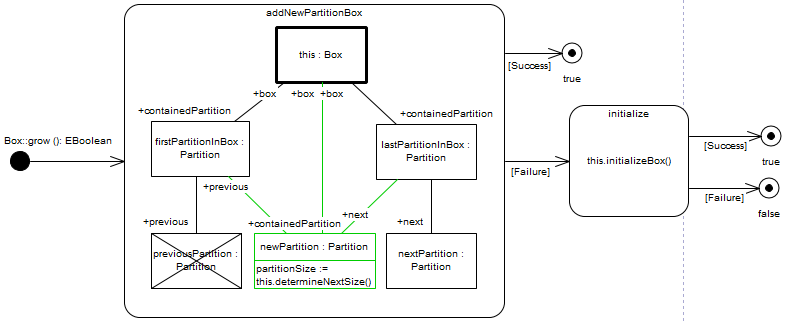
\includegraphics[width=\textwidth]{ea_growAdditions}
  \caption{Extending \texttt{grow} with a \emph{MethodCallExpression}}
  \label{fig:newGrowControl}
\end{center}
\end{figure}

\clearpage

\item[$\blacktriangleright$] Switch back to your open \texttt{Box.grow} SDM in EA. You'll notice that if you double-click on \texttt{initialize}, the
\texttt{Extract Story Pattern} option is invalid. This makes sense -- you don't define a pattern in a statement node. Instead, return to the main diagram and
create a new SDM for \texttt{initializeBox}.

\item[$\blacktriangleright$] In its diagram, create an \texttt{activity node} named \texttt{buildPartitions}. Within it, have a bound \texttt{Box} linked to a
\texttt{onePartition} NAC, and two other `green' (create) object variables, \texttt{firstPartition} and \texttt{lastPartition}. Be sure to also connect two
true/false \texttt{StopNode}s. The pattern should now resemble Fig.~\ref{fig:buildPartitions}. The NAC here can only fulfilled if the box has no partitions,
i.e., is in a pristine state and able to be initialized. In other words, If \texttt{grow} is used for an empty box, it initializes the box for the first time
and grows it after that, ensuring that the box is always in a valid state.

\vspace{0.5cm}
 
\begin{figure}[htp]
\begin{center}
  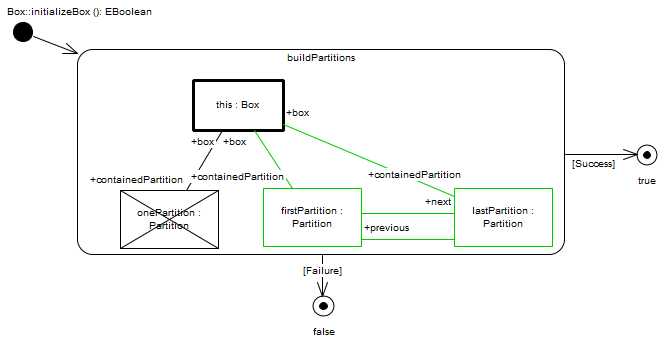
\includegraphics[width=\textwidth]{eclipse_buildPartitions}
  \caption{Compelted NAC to check for \emph{one} partition}
  \label{fig:buildPartitions}
\end{center}
\end{figure}
 
\item[$\blacktriangleright$] You're finished! Save, validate, and build your metamodel, then check out how this is done in the textual syntax in
Fig.~\ref{fig:updateGrow} and Fig.~\ref{fig:pattBuildParts}.

\jumpSingle{initialize notes}

\end{itemize}
